\documentclass[12pt]{article}

\usepackage{tgtermes}
\usepackage{epsf}
\usepackage{epstopdf}
\usepackage{amsmath}
\usepackage{graphicx}
\usepackage{booktabs}
\usepackage[colorlinks=true,linkcolor=blue,citecolor=blue]{hyperref}
\usepackage{dcolumn}
\usepackage{amsmath, amsthm, amssymb}
\usepackage{mwe}
\usepackage{url}
%\usepackage{harvard}
\usepackage{fancyheadings}
\usepackage{longtable}
\usepackage{authblk}
\usepackage{setspace}
%\usepackage[nomarkers]{endfloat}
\usepackage{float}
\usepackage{bbm}
%\usepackage{titling}
\usepackage{subcaption}
\usepackage{algorithm}
\usepackage{algorithmic}
\usepackage{import}
\usepackage[backend=biber,style=authoryear,
sorting=ynt,citestyle=authoryear]{biblatex}
\addbibresource{papercitations.bib}
%\usepackage[nomarkers,nofiglist,notablist]{endfloat}
\usepackage{subcaption}
\usepackage{caption}

\onehalfspacing
\textwidth 6.5in \oddsidemargin 0in \evensidemargin -0.6in
\textheight 8.5in \topmargin -0.2in

\newcolumntype{L}[1]{>{\raggedright\let\newline\\
		\arraybackslash\hspace{0pt}}m{#1}}
\newcolumntype{C}[1]{>{\centering\let\newline\\
		\arraybackslash\hspace{0pt}}m{#1}}
\newcolumntype{R}[1]{>{\raggedleft\let\newline\\
		\arraybackslash\hspace{0pt}}m{#1}}
\newcolumntype{P}[1]{>{\raggedright\tabularxbackslash}p{#1}}

\newtheorem{theorem}{Theorem}[section]
\newtheorem{corollary}[theorem]{Corollary}
\newtheorem{proposition}[theorem]{Proposition}
\newtheorem{lemma}[theorem]{Lemma}

\captionsetup{justification=centering,singlelinecheck=false}


\newcommand{\xsub}[1]{%
	\mbox{\scriptsize\begin{tabular}{@{}c@{}}#1\end{tabular}}%
}

%\renewcommand{\thetable}{\Roman{table}}

\begin{document}
	
	
	
	
	\linespread{1.2}\title{\vspace{-0.5in} Does Hospital Leadership Matter?\\ \large Evidence from Pay-for-Performance Incentives} 
	
	\date{\today}
	
	\author{\vspace{10mm}Hanna Glenn\footnote{Department of Economics, Emory University, 1602 Fishburne Drive, Atlanta, GA 30322, hanna.glenn@emory.edu.} }
	
	\maketitle
	%\setlength{\droptitle}{-10pt}
	
	\vspace{-0.2in}
	
	\singlespacing\maketitle


 \vspace{3mm}
	
    \begin{abstract}
		{\small
         Firm leaders are shown to be correlated with firm decisions and performance. In this paper, I investigate this topic in the context of hospital executive teams. Specifically, I empirically the effect of clinically trained executives on hospital behavior in response to an incentive shock. In particular, I leverage policies changing quality incentives for hospitals in the US in 2012, and estimate the difference in readmission and mortality rate responses for nonprofit hospitals with and without clinically trained executives. I find that a lack of clinical executives leads hospitals to improve quality more drastically after the incentive change. Further, I provide evidence that the more drastic response is due to non-clinical executives being more profit driven, and that clinical executives are not just a signal of underlying hospital objectives, but manage the hospital differently. 
		} 
	\end{abstract}
	
	
	
	
	\vspace{0.8in}
	
	\noindent Keywords: 
	
	\noindent JEL Codes: 
	
	\onehalfspacing
	
	\newpage

    Various characteristics of firm leadership such as gender, age, and background have been shown to be correlated with firm decisions and performance. I investigate this topic in the context of hospital executives with differing backgrounds: some with training as a medical doctor and some without. Hiring physician executives can be controversial. On one hand, physicians bring a unique combination of clinical and administration expertise, and they have insights that can potentially improve hospital outcomes (\cite{Stajduhar_2023}, \cite{Ahmed_2022}). Alternatively, physicians may not always be adequately trained to enter into high level management positions, and therefore worsen hospital outcomes (\cite{HarvardBusinessReview2018}). In this paper, I investigate how having clinically trained executives in leadership affects hospital response to pay-for-performance incentives.  

    I scrape executive team names and titles from publicly available Tax Form 990s, filled out by nonprofit firms in the US. Combining this with publicly available hospital characteristics, I construct a novel data set of nonprofit hospitals from 2010-2014 containing information on both executive team characteristics and quality metrics. Nonprofit behavior in the hospital industry directly affects health care consumers, as private nonprofit hospitals make up 50\% of all hospitals in the US, and staff, on average, 207 beds. For comparison, for-profits make up 36\% of hospitals and staff 107 beds (\cite{ASPE_2023}). 
    
    The selection of leaders makes it difficult to interpret any direct comparison of differing executive teams as causal. Therefore, I leverage an exogenous shock to hospital incentives, pay-for-performance policies enacted in the US in 2012, and compare the change in readmission and mortality rates of executive teams with and without clinical executives. Under the assumption that the two types of teams would have had similar trends in readmission and mortality rates absent the incentive change, I find that a lack of clinically trained executives leads a hospital to respond more drastically to pay-for-performance incentives. 
    
    Having found that hospital leadership does, in fact, matter to hospital behavior, I investigate several mechanisms that might contribute to this difference. First, \textcolor{red}{the more drastic decrease in readmissions by nonclinical teams is not driven by decreasing average patient complexity. There is no difference in patient case mix between clinical and nonclinical executive teams}. Further, I comparing each type of leadership team with for-profit hospitals reveals that the absence of clinical executives leads a nonprofit hospital to respond more similarly to a for-profit hospital. That is, having clinical training on a leadership team leads a hospital to act less profit-driven than their general training counterparts. Finally, I show that changes in a hospital's propensity to hire a clinical executive are not correlated with the pay-for-performance policies. Thus, I exploit such changes in leadership teams to decompose the effect of clinical executives into signaling (clinical executives signal underlying hospital preferences), or managing (clinical executives manage the hospital differently). I find that the entire difference in response is driven by a managing effect. 

    Many researchers have documented a correlation between executive characteristics, specifically for CEOs, and firm performance, starting with \citeauthor{bertrand2003managing} (\citeyear{bertrand2003managing}), who show that manager fixed effects are an important driver of many firm behaviors and decisions. Female board members are associated with better oversight and more women executives (\cite{matsa2011chipping}; \cite{adams2009women}), but are negatively correlated with firm value (\cite{ahern2012changing}). Having more female executives is correlated with female employee wages and corporate strategies (\cite{flabbi2019female}; \cite{matsa2013female}); young male CEOs tend to be more aggressive in mergers and acquisitions, while those with military experience are less aggressive (\cite{levi2010deal}; \cite{benmelech2015military}); CEOs with general ability tend to receive higher pay and perform better (\cite{kaplan2012ceo}; \cite{custodio2013generalists}; \cite{adams2018director}; \cite{frydman2019rising}). Further, Chief Diversity Officers are not found to have any effect on hiring more diversely in universities (\cite{bradley2022impact}). 
    
    Due to data limitations, many of these studies focus on large, publicly traded firms in the US. \citeauthor{brickley2010board} (\citeyear{brickley2010board}) has the only study to my knowledge answering this question in the US nonprofit context. Using exogenous variation in expected Medicare profits, the authors find that having an internal board of directors increases CEO compensation, and having physician board members decreases public donations (\cite{brickley2010board}). Additionally, two studies focus on hospital performance in other countries. \citeauthor{janke2019impact} (\citeyear{janke2019impact}) uses data from England to study whether CEOs affect hospital production, and find no association (\cite{janke2019impact}). However, \citeauthor{otero2022managers} (\citeyear{otero2022managers}) investigates the role of CEOs in public hospitals in Chile, and finds an 8\% decrease in mortality rates for hospitals with top managers. Further, a major contributor of this quality improvement is the exodus of older physicians as CEOs (\cite{otero2022managers}). I contribute to our knowledge of how executive team characteristics affect firm behaviors by (1) considering the important setting of nonprofit hospitals, which serve the majority of patients in the US, (2) considering a unique executive characteristic which is plausibly relevant, and (3) observing firm behavior in the presence of an exogenous incentive change. 

    Additionally, I contribute to our understanding of how providers respond to pay-for-performance incentives in health care. The most in depth study of how hospitals respond to the Hospital Readmissions Reduction Program, one of the two large pay-for-performance initiatives, is \citeauthor{gupta2021impacts} (\citeyear{gupta2021impacts}). This study finds that hospitals decreased readmissions by 5\% and mortality rates by 2\% on average as a result of the program, confirming prior studies (\cite{mellor2017does}; \cite{ziedan2018essays}; \cite{ody2019decreases}; \cite{gupta2021impacts}). Around 40\% of the decrease in readmissions is due to selective patient practices. Further, market concentration and hospital systems play a large role in how hospitals respond to the program (\cite{kunz2024assessing}). Research on the other large pay-for-performance initiative, the Hospital Value Based Purchasing Program, generally finds that the program had no effect on underlying hospital quality (\cite{us2015hospital}; \cite{norton2018moneyball}; \cite{friedson2019so}). This paper contributes to our understanding of how characteristics of hospitals affect response to pay-for-performance incentives.

    \section{Setting and Data}

    \subsection{Nonprofit Hospital Executives}

    Nonprofit firms in the US differ from for-profits mainly in that for-profit firms distribute revenue to stakeholders, while nonprofits reinvest profit back into the firm. Hospitals are governed by a board of directors, whose role is to set broad goals and strategies, and provide general oversight. The board selects executives, the highest level of management of a firm, to carry out day-to-day operations. An executive team usually consists of at least a Chief Executive Officer (CEO) and Chief Financial Officer (CFO), but there is variation in how firms organize executive teams. Some hospital executives to specialize in health care settings by earning a degree in health care management, or an MBA specific to health care. There are executive positions that are often filled by someone with clinical training, such as a Chief Medical Officer (CMO), but medical doctors can pursue other top managerial positions as well such as CEO or president. While some doctors earn additional degrees before stepping into an executive role, this is not a necessary condition to becoming a physician executive. 

    Hospital executive teams are understudied partly due to the inaccessibility of granular data. I construct a novel data set of not-for-profit hospitals in the US that contains names, titles, and positions of all board members and executives tied to the hospital from 2009-2015. I gather this data from publicly available Tax Form 990s, which every sufficiently large nonprofit files each year in the US. To my knowledge, this is the first large scale gathering of executive names from these forms.\footnote{\citeauthor{brickley2010board} (\citeyear{brickley2010board}) collects compensation data for a select number of hospitals.} 

    All tax-exempt organizations in the US are required to file a Form 990 with Internal Revenue Services (IRS) each year. There are different types of forms, but any organization grossing over \$200,000 must file the most extensive Form 990. Sections of this form include a statement of revenue, statement of functional expenses, a balance sheet, and, as used in this project, a list of all key employees, executives, and board members. Each firm is required to report the name and title, average hours per week, position, and compensation of their board members and executives. 

    The historical tax forms for all not-for-profits are housed by ProPublica.\footnote{https://projects.propublica.org/not-for-profits/} I use the NonProfit Explorer API to extract Employee Identification Numbers (EIN) of NFPs with a hospital National Taxonomy of Exempt Entities (NTEE) code. After filtering out associations and specialty hospitals, there are approximately 3,000 NFP EINs. Linking these EINs to other hospital information is crucial for the analysis. I therefore rely on matching by location and name of hospital in both the tax forms and AHA data. In the AHA data, I limit to general hospitals. Then, I confidently match 1200 EINs to an AHA identification number based on exact name matches within the same state. I assess the observable differences between matched and non-matched hospitals in Appendix \ref{app:matched}, and conclude that the samples are overall similar apart from an under-sampling of hospitals that belong to systems.
    
    For each of the matched EINs, I extract web URLs to Form 990 PDFs for each year. I use an algorithm to download these locally and use optical character recognition (OCR) text extraction methods to scrape the relevant section of the PDF, which is titled ``Officers, Directors, Trustees, Key Employees, and Highest Compensated Employees". Finally, I use string cleaning methods to identify all names and positions under each EIN, year. With each name, I extract titles indicating clinical training: MD, Dr., or DO. Using OCR extraction can be unreliable in cases where the text on the form is handwritten or small. Therefore, for observations that are missing after the initial extraction, I manually record names, positions, and titles. As I limit the sample to hospitals who have text information in every year, I limit the years to 2010-2014 to retain more hospitals. This yields 852 not-for-profit hospitals that are matched to AHA data, and with complete text information in each year. 

    Finally, I match each name with the National Plan and Provider Enumeration System (NPPES) database of all registered physicians. The goal is to match each physician with an NPI number in order to merge publicly available data on physician specialty, gender, and tenure. For any person who has a doctor title and uniquely matches the NPPES data, I record their NPI number. For anyone who has a doctor title and no matches, no doctor title and matches, or a doctor title and multiple matches, I use information on location and hospital name to manually match the NPI. 

    For the purposes of this paper, I focus on executive teams as a whole instead of specific positions. The main reason for this is because the organization of teams varies so drastically across hospitals that a specific position, even if it exists in two different hospitals, can be meaningfully different. I drop anyone who is solely a board member, and focus on those who have executive in their title, or are labeled as a president or vice president of a department. I create various hospital-level characterizations based on their executive team, such as the existence of a clinically trained executive, the number of clinically trained executives, the number of total executives, and whether the hospital has a Chief Medical Officer. For my main sample, I limit to hospitals who do not change their propensity to hire a clinical executive for the duration of the sample. Summary statistics for these variables are shown in Table \ref{leader_sumstats}. On average, NFP hospitals in my sample have 4 executives and .4 clinically trained executives. Sixty-one percent of the sample never changes propensity to hire a clinically trained executive, and 33\% of NFPs in the sample have a Chief Medical Officer at some point. 

     \import{Tables}{leader_sumstats.tex}
  
    \subsection{Pay-for-Performance Policies Targeting Readmission and Mortality Rates}\label{sec:hrrp}

    Two programs were passed as part of the Affordable Care Act that focused on pay-for-performance incentives for hospitals: the Hospital Readmissions Reduction Program (HRRP), and the Hospital Value Based Purchasing Program (HVBP). HRRP focused on penalizing hospitals with poor quality, and HVBP focused on rewarding hospitals with high quality or show improvement in quality. 

    In October 2011, the Center for Medicare and Medicaid Services (CMS) released a set of rules under HRRP mandating penalties for hospitals with above average readmission rates. The goal of HRRP is to lower readmissions through better care coordination, less initial stay complications, and better post-care instructions. Beginning in October 2012, hospitals with higher readmission rates than the national average in pneumonia, heart failure, or AMI (after adjusting for demographic characteristics) receive a fixed lower reimbursement rate for all Medicare patients seen in their hospital. In 2015, CMS also included chronic obstructive pulmonary disease, coronary artery bypass graft surgery, and elective primary total hip arthroplasty and/or total knee arthroplasty as conditions which go into the penalty calculation (\cite{CMS}). 
    
    Penalties are given in the form of a fixed rate reduction of 1-3\% for every Medicare patient regardless of the condition. Further, CMS does not distinguish a necessary readmission from an avoidable readmission; any repeat hospital visit is included in the penalty calculation. Excess readmission rates are calculated using a rolling look-back period of 3 years to determine whether the hospital is penalized. Therefore, hospitals had incentive to react immediately once details of the program were announced in October of 2011. 

    The HVBP Program instead rewards hospitals with high quality or significant improvement in quality. Specifically, CMS deducts Medicare payments by 2\% from all eligible hospitals, collects this sum, and divides it among the rewarded hospitals. Several quality and cost measures surrounding safety, efficiency, cost reductions, clinical outcomes, and community engagement are combined to create a single score metric for each hospital. Hospitals are then compared to the average and are rewarded for being above average quality or for showing improvement (\cite{CMS_2023}). 

    Therefore, I focus on outcomes of readmission and mortality rates, which are publicly available at the hospital-condition level in CMS Hospital Compare. I combine rates for pneumonia, AMI, and heart failure (the relevant HRRP conditions) into a weighted average based on the number of patients in each condition. Additionally, I include several relevant hospital characteristics from the AHA survey: number of beds, and whether the hospital is an academic medical center, is physician owned, or is system affiliated. Additionally, case mix index, a measure of overall patient complexity, comes from the CMS Case Mix Index files. Whether the hospital was penalized under HRRP or received payments under HVBP is found in the HCRIS data. 

	\subsection{Summary Statistics}\label{sec:data}

    In Table \ref{tab:sumstats_samples}, I present a table of means of relevant variables for several hospital samples used throughout the analysis. First, there are 708 for-profit hospitals in the sample, shown in column (1). For-profit hospitals in the sample have 155 beds on average, 112-276 patients depending on the condition, and are highly likely to be affiliated with a system. Thirty six percent of for-profits were penalized for all three conditions at some point. 

    \import{Tables}{sample_sumstats.tex}

    Columns 2-4 show variable means for not-for-profits in the sample, with all NFPs in column 2, NFPs that ever have a clinically trained executive in column 3, and NFPs that never have a clinically trained executive in column 4. NFPs are much less likely to be physician owned or system affiliated compared to FPs. They do, however, have similar bed size and case mix index to FPs. Twenty-two percent of all NFPs are penalized for all conditions. There are several differences among NFPs with and without clinically trained executives. Those with a clinically trained executive are larger in terms of beds and patients seen, are more likely to be an academic medical center, and see slightly more complex patients. Further, they are more likely to be penalized for every condition. 

    Finally, columns 5-6 limit the sample of not-for-profits further using changes in executive teams. The NFPs included in this sample do not change their propensity to hire a clinically trained executive, they either always have the same number of clinically trained executives or always have no clinically trained executives. The differences in NFPs with and without clinically trained executives remains similar with this sample limitation. I discuss the implications of these differences for identification in Section \ref{sec:model}. 

    I plot weighted average readmission and mortality rates across time for different hospital types in Figure \ref{fig:weighted_read_mort_graph}, where I adjust both rates by baseline patient complexity. Pay-for-performance incentive changes are shown as a dotted line between 2011 and 2012. For-profit hospitals have the highest readmission rates prior to 2012. While the readmission rate trend behaves similarly across hospital types prior to the programs, there are notable trend differences after the programs. For-profits decrease readmissions drastically. NFP trends depend on the presence of an executive MD, where those without a clinically trained executive respond drastically, more similarly to for-profits, than those with a clinically trained executive. In mortality rates, NFPs with a clinically trained executive have the lowest rates before the programs, but differentially continue with an increasing trend in mortality after the programs. While this is purely descriptive evidence, the trends in outcomes point to more similar behavior between for-profits and NFPs without a clinically trained executive in comparison to NFPs with a clinically trained executive.

    \begin{figure}[ht!]
    \centering
        \caption{Outcomes Over Time}
        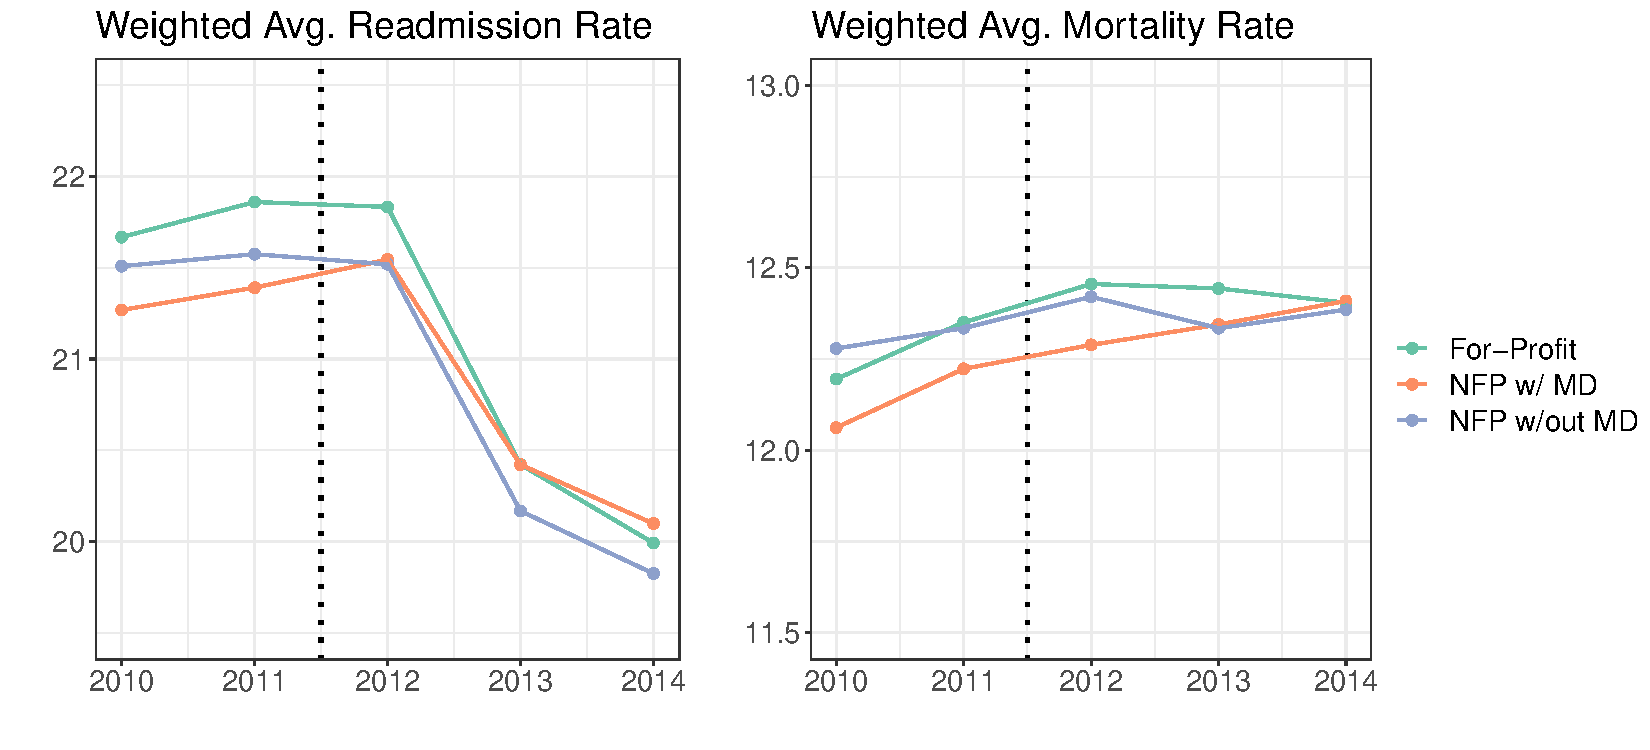
\includegraphics[width=\textwidth]{Objects/weighted_read_mort_adjusted_graph.pdf}
        \label{fig:weighted_read_mort_graph}
    \end{figure}


    \section{Effect of Executive Clinical Training on Hospital Response}\label{sec:clinical}

    My first goal is to estimate the effect of having clinical executive training on how hospitals change readmission and mortality rates in response to pay-for-performance incentives. Ultimately, I employ synthetic difference-in-differences, weighting more heavily non-clinical hospitals with readmission, mortality, and baseline case mix index that better match the clinical team trends. However, for clarity, I present the unweighted specification:

    \begin{equation}
    \label{eq:clinical}
    y_{ht} = \beta \text{ (clinical training x post 2012)}_{ht} + \gamma_{h} + \delta_t + \epsilon_{ht},
    \end{equation}
    

    \noindent where $y_{ht}$ is one of the outcome variables discussed in Section \ref{sec:hrrp}, and $\gamma_h$ and $\delta_t$ are hospital and time fixed effects, respectively. 

     I rely on several assumptions to identify this effect. First, I assume that, absent the program enactments, hospitals with different leadership team characterization types would have behaved similarly in outcomes. While I see no evidence of pre-trends, Table \ref{tab:sumstats_samples} suggests that hospitals with a clinically trained executive are different than other hospitals along multiple characteristics. There may be concern that these differences between hospital types could be driving the results. Therefore, my main specification uses the synthetic difference-in-differences method established in \citeauthor{arkhangelsky2021synthetic} (\citeyear{arkhangelsky2021synthetic}). This method creates unit weights that more heavily factor comparison hospitals that are similar to the treat group hospitals prior to the programs. It also weighs time periods that balance pre-programs and post-programs for the comparison hospitals. Then, a simple two way fixed effects estimator is used with these weights, yielding a more robust average treatment effect that relies less on a strong parallel trends assumption (\cite{arkhangelsky2021synthetic}). I present the synthetic diff-in-diff estimates as the main results, and they are largely similar to the standard two way fixed effects results with no weights, shown in Appendix \ref{app:fullsample}. Further, the conceptual identification is the same as a standard difference-in-differences.

    \subsection{Results}

    The estimated difference in readmission rate trends for all hospital types in response to the programs are shown in Figure \ref{fig:clinicalsynthdid}. In panel \ref{fig:read_synth_clinical}, I compare readmission rate responses among nonprofit hospitals with and without clinical training on their executive team. Estimate $\beta$ is represented in the difference in slope after 2012 when pay-for-performance incentives began. Nonprofits without a clinically trained executive lowered readmission rates by .24 ppts more than those with a clinically trained executive. 

    I also directly estimate the difference in mortality rates among NFPs with and without clinical experience in panel \ref{fig:mort_synth_clinical}. Again, the difference is not statistically significant, but the coefficient compared to the true nulls in panels \ref{fig:mort_synth_clinical} and \ref{fig:mort_synth_plotc} indicates NFPs without a clinical executive potentially decrease mortality more aggressively than NFPs with a clinical executive. In Appendix \ref{app:condition}, I show that these results are mainly driven by pneumonia patients.  


     \begin{figure}
     \caption{Effect of Clinical Experience on Readmission and Mortality Rates}
     \centering
     \begin{subfigure}[b]{0.45\textwidth}
         \centering
         \caption{Readmission Rate}
         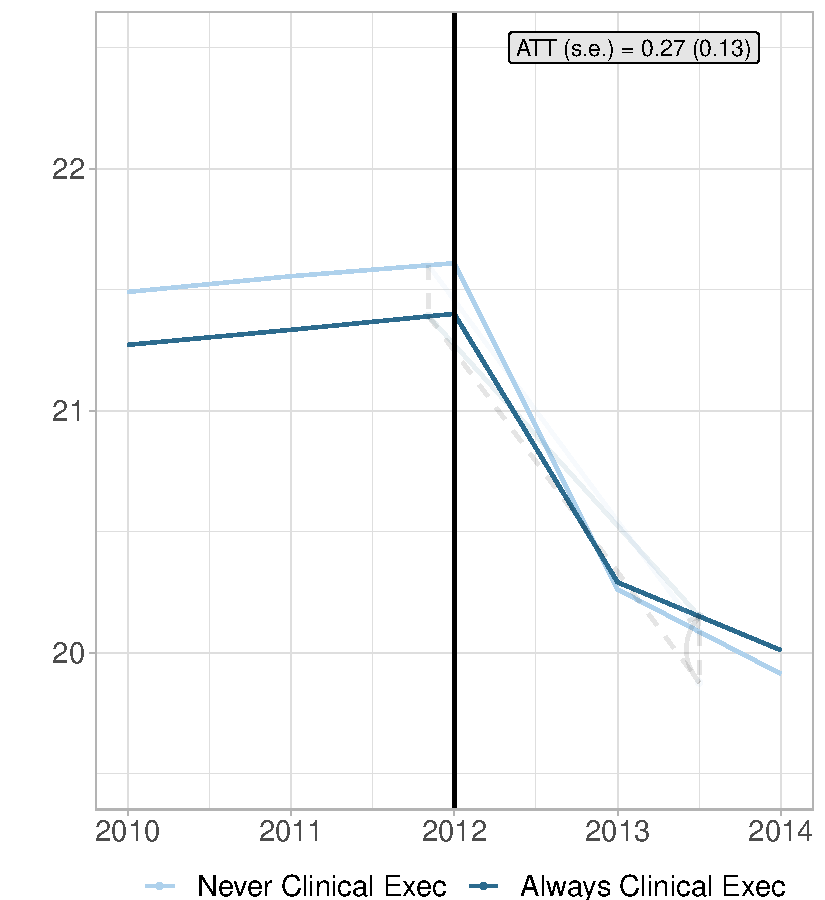
\includegraphics[width=\textwidth]{Objects/read_md_nomd_synth_graph.pdf}
         \label{fig:read_synth_clinical}
     \end{subfigure}
     \hfill
     \begin{subfigure}[b]{0.45\textwidth}
         \centering
         \caption{Mortality Rate}
         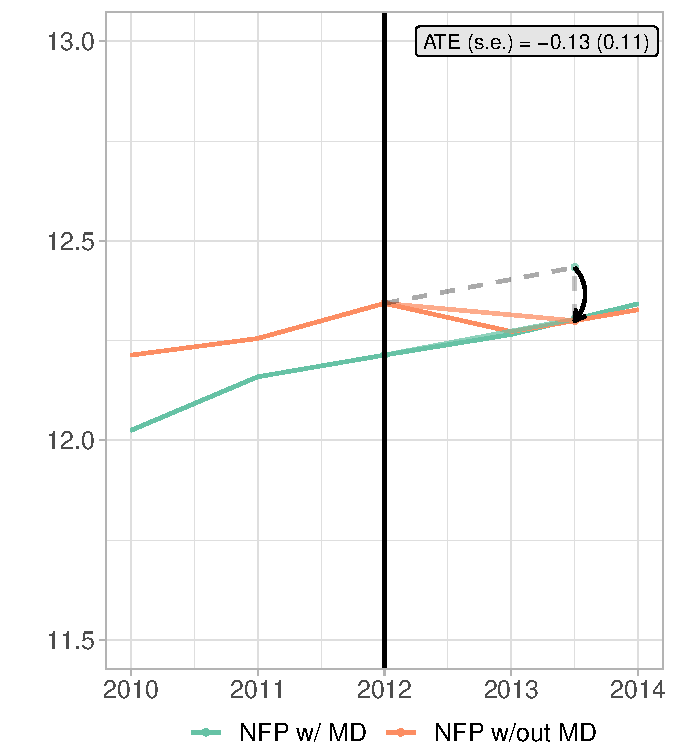
\includegraphics[width=\textwidth]{Objects/mort_md_nomd_synth_graph.pdf}
         \label{fig:mort_synth_clinical}
     \end{subfigure}
        \label{fig:clinicalsynthdid}
    \end{figure}


    \section{Are Clinical Executives less Profit Driven?}\label{sec:forprofit}

    A reason for the difference in hospital behavior with the presence of clinically trained executives could be how profit-driven a physician vs. a general leader is. To demonstrate this, consider hospital behavior under the enactment of pay-for-performance policies, where hospitals face a trade-off between profit and societal benefit. Pay-for-performance incentives essentially incorporate quality directly into a hospital's profit function (\cite{dranove2011health}), whereas a fee-for-service system only incentivizes quantity. A hospital that places all value on profit will only care about quality when it enters into the profit function, and therefore will respond more drastically to pay-for-performance than a hospital who already cared about quality through societal benefit before the incentives.\footnote{I present the theoretical model and mathematical results in Appendix \ref{sec:model}.} Therefore, observing hospital responses to pay-for-performance incentives reveals information about their underlying preferences.  

    I compare readmission and mortality rates of each nonprofit leadership team type to for-profit hospitals. Since for-profit hospitals have revealed through their ownership status that they are largely profit-driven, comparing different executive team behavior to for-profit behavior helps reveal how profit driven certain leadership teams are. Thus, I estimate

    \begin{equation}
    \label{eq:forprofit}
    y_{ht} = \beta \text{ (for-profit x post 2012)}_{ht} + \gamma_{h} + \delta_t + \epsilon_{ht},
    \end{equation}

    \noindent for two subsets of data. First, I limit only to for-profits and nonprofits with clinical leadership. Second, I limit only to for-profits and nonprofits without clinical leadership. Thus, $\beta$ represents the effect of being for-profit compared to being nonprofit with a certain leadership team type.

    The identification assumptions I make here are largely similar to those in the main analysis, only now incorporate for-profit hospitals. First, I assume that, absent the change in incentives, for-profit and the relevant comparison group would have had parallel trends in outcomes. While this is not directly testable, both the synthetic difference in difference and event studies indicate parallel trends prior to the incentive changes. Second, I assume that the stability of nonprofit leadership teams is not correlated with the 2012 policy changes. I explore this assumption in Section \ref{sec:identification}. I also assume that there is no anticipation of the policy changes prior to 2012, which is reasonable as the rules of the policies were announced in October of 2011. Finally, I assume no other changes correlated with both hospital type (for-profit, nonprofit with and without clinically trained executives) and quality occurred in conjunction with the 2012 pay-for-performance policies.

    The estimates and graphical representation of the effect of being for-profit is shown in Figure \ref{fig:read_synth_plot}. In panel \ref{fig:read_synth_plotb}, the average treatment effect represents the effect of being for-profit compared to nonprofit with clinical executives on readmission rates after pay-for-performance changes. While readmission rates trend similarly prior to the incentive change, for-profits decrease readmission rates by .3 more than nonprofits with clinically trained executives. That is, for-profits respond more aggressively to the incentive change than nonprofits with clinical leadership. However, panel \ref{fig:read_synth_plotc} shows no such difference when comparing for-profits to nonprofits without clinically trained executives. Not only is the estimate not statistically significant, but the magnitude indicates a precise zero. That is, a lack of clinically trained executives leads nonprofits to act like for-profits in terms of readmission rates when responding to this incentive change. 

 \begin{figure}[ht!]
     \caption{Readmission Rate Synthetic Difference in Differences Results}
     \centering
     \begin{subfigure}[b]{0.45\textwidth}
         \centering
         \caption{For-Profit and NFP w/ MD Exec}
         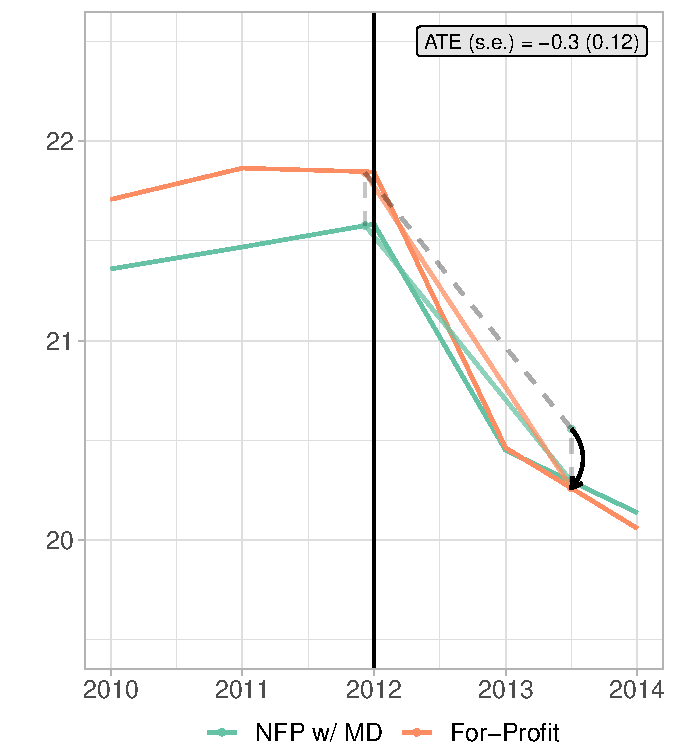
\includegraphics[width=\textwidth]{Objects/read_fp_md_synth_graph.pdf}
         \label{fig:read_synth_plotb}
     \end{subfigure}%
     \vspace{5mm}
     \hfill
     \begin{subfigure}[b]{0.45\textwidth}
         \centering
         \caption{For-Profit and NFP w/out MD Exec}
         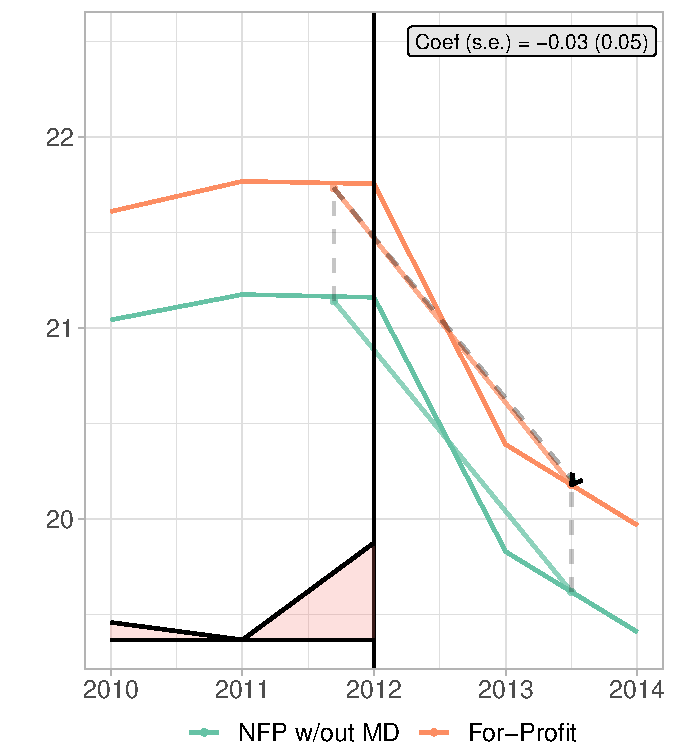
\includegraphics[width=\textwidth]{Objects/read_fp_nomd_synth_graph.pdf}
         \label{fig:read_synth_plotc}
     \end{subfigure}
        \label{fig:read_synth_plot}
    \end{figure}

    

    Next, I present estimated differences in mortality rates between different hospital types in Figure \ref{fig:mort_synth_plot}. In panel \ref{fig:mort_synth_plotb}, the estimated difference is between for-profits and nonprofits with clinically trained executives. The magnitude of the difference in mortality rates is .11, where only for-profits seem to be reacting to the incentive change. While still statistically insignificant, I argue that this still indicates a difference in behavior between the hospital types, particularly due to the documented noisiness of mortality measures (\cite{mackenzie2016measuring}). However, the estimated difference in mortality between for-profits and nonprofits without clinically trained executives is certainly zero. 


    \begin{figure}[ht!]
     \caption{Mortality Rate Synthetic Difference in Differences Results}
     \centering
     \begin{subfigure}[b]{0.45\textwidth}
         \centering
         \caption{For-Profit and NFP w/ MD Exec}
         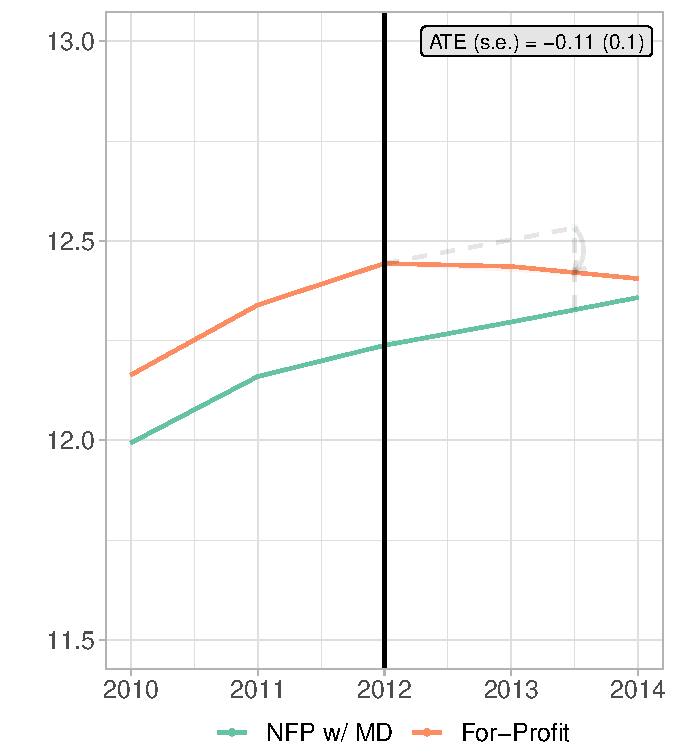
\includegraphics[width=\textwidth]{Objects/mort_fp_md_synth_graph.pdf}
         \label{fig:mort_synth_plotb}
     \end{subfigure}%
     \hfill
     \begin{subfigure}[b]{0.45\textwidth}
         \centering
         \caption{For-Profit and NFP w/out MD Exec}
         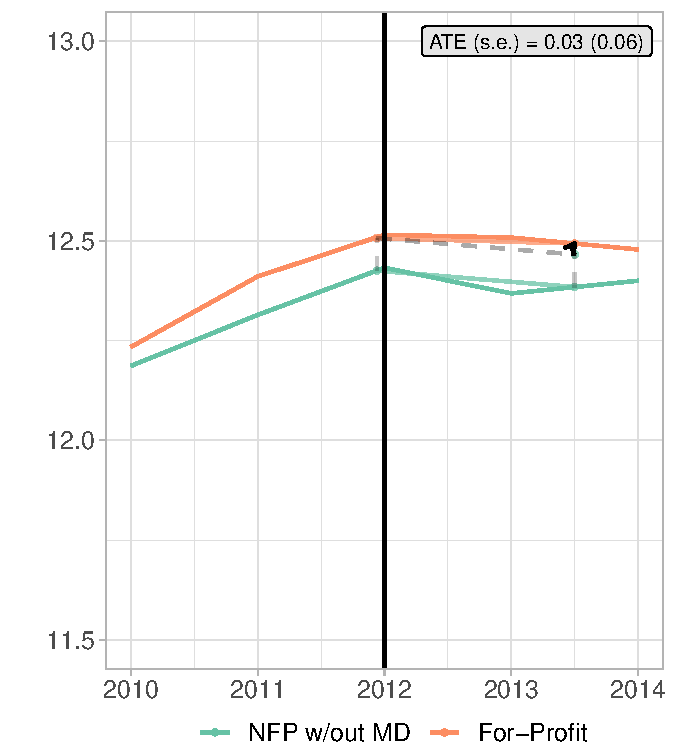
\includegraphics[width=\textwidth]{Objects/mort_fp_nomd_synth_graph.pdf}
         \label{fig:mort_synth_plotc}
     \end{subfigure}
        \label{fig:mort_synth_plot}
    \end{figure}
    

\section{Signaling vs. Managing Decomposition}

    To this point, I have limited the sample of nonprofit hospitals to those that don't change their propensity to hire a clinically trained executive over the sample period. However, under the assumption that hiring or firing these types of executives is not correlated with the pay-for-performance policy changes, these changes can be leveraged to understand further how executive characteristics affect hospital behavior. Particularly, a clinically trained executive could be a signal of the underlying objectives of the hospital, or hiring a clinically trained executive who carries out day-to-day operations in a distinct way effectively changes the objectives of the hospital. 

    To disentangle the two, I carefully define the ``treat" and comparison group of hospitals in the following estimating equation. For clarity, I present the specification details in Figure \ref{fig:decomp_spec}. If clinically trained leaders are simply signals of underlying objectives, it shouldn't matter when hospitals have hired a clinical executive. For example, take two hypothetical hospitals. Hospital A has a clinically trained executive from 2010-2011. Hospital B has a clinical executive from 2010-2013. If clinically trained executives are a signal of underlying objectives, these two hospitals should respond similarly to pay-for-performance objectives despite only one of them having a clinical executive in 2012. However, if clinically trained leaders manage the hospital in a unique way, these two hospitals would respond differently since only one of them has clinical leadership in 2012 when the policy changes occurred. 

    \begin{equation}
    \label{eq:decomp}
    y_{ht} = \beta \text{ (treat x post 2012)}_{ht} + \gamma_{h} + \delta_t + \epsilon_{ht},
    \end{equation}
    

\begin{figure}[ht!]
\begin{center}
\caption{\label{fig:decomp_spec}Decomposition Model Specification Details}
 
 \begin{tabular}{| m{18em} |}
 \hline
 Signaling:\\ [0.5ex]
 \hline\hline 
 \vspace{2mm}
 Treat Group:  \hspace{15mm} Never MD \\
 \vspace{2mm}
 Comparison Group: \hspace{3mm} Ever MD  \\
 [1ex]
 \hline
 \end{tabular}
\hfil   %<---
 \begin{tabular}{|m{18em}|}
 \hline
 Managing:\\ [0.5ex]
 \hline\hline
 \vspace{2mm}
 Treat Group: \hspace{11mm} No MD in 2012 \\
 \vspace{2mm}
 Comparison Group:  Ever MD (not in 2012)  \\
 [1ex]
 \hline
 \end{tabular}
 
\end{center}
 \end{figure}



    I have discussed the assumptions of parallel trends, no anticipation, and no other confounding events in both Sections \ref{sec:clinical} and \ref{sec:forprofit}. These assumptions are also necessary here. In those Sections, I have discussed that stability of leadership team must not be correlated with the 2012 policy changes. Up to this point, that assumption was important because of the way I selected the sample. However, this decomposition depends directly on leveraging such leadership changes. Thus, I now explore this assumption in detail. 

     I assess the validity of the exogenous changes assumption in two ways. First, I analyze whether changes in clinically trained executives occur more often in time periods of program enactment. Second, I analyze whether hospitals who end up getting penalized or receiving payments are more likely to make changes in clinical executive members than those who are not. That is, are hospitals that expect to be affected by the programs more likely to hire or fire clinically trained executives? I consider changes in having any clinically trained executive, as well as changes in the number of clinically trained executives. I estimate the following linear equations:

    \begin{equation}\label{eq:change1}
    \text{change}_{ht} = \sum_{j=2011}^{2014}\beta_j\mathbf{1}\{t=j\} + \alpha_h + \epsilon_{ht},
    \end{equation}

    \begin{equation}\label{eq:change2}
    \text{change}_{ht} = \beta(\text{Program Exposed}_{h} \times \text{Post Programs}_t)+ \alpha_h + \delta_t + \epsilon_{ht}.
    \end{equation}

    The variable $\text{Program Exposed}_{h}$ is an indicator for whether the hospital eventually was penalized under HRRP or received payments under HVBP. The estimates from this analysis are presented in Table \ref{tab:change_analysis}. Changes in any clinically trained executive are less likely to occur in 2012-2014 relative to 2010, indicating that executive teams are actually becoming more stable over time along the dimension of hiring clinically trained executives. Further, hospitals who end up being penalized through HRRP or receiving payments through HVBP are not more likely to change their propensity to hire any clinically trained executive. Results are similar when considering changes in the number of clinically trained executives. Thus, it seems unlikely that endogenous team formation is biasing the estimates. In Appendix \ref{app:changes}, I present various descriptive statistics of executive team changes over time, showing that hiring and firing of MD executives do not change much over time, the rate of clinical executives to total executives remains stable over time, and the distribution of timing of clinical executive changes. 

     \import{Tables}{change_analysis.tex}

    The estimates of each decomposition specification are shown in Table \ref{tab:MD_noMD_readmort_decomp_synth}. Columns (1) and (2) show that the difference in readmission response is driven by having a clinically trained executive in 2012, compared to having a clinically trained executive at another point in time. Columns (3) and (4) support the same theory given the magnitudes of the coefficients, but are still statistically insignificant due to the noisiness of mortality. The results suggest that managers make a difference in behavior and objectives, rather than being a signal of already existing objectives. 

    \import{Tables}{MD_noMD_readmort_decomp_synth.tex}


    \section{Conclusion}

    Existing literature is inconclusive as to whether not-for-profit (NFP) hospitals differ meaningfully from for-profit hospitals. NFP objectives have direct implications for patients, yet are largely unknown. An observable and economically meaningful characteristic of NFP hospitals that may affect underlying objectives is the composition of the hospital's top management. Particularly, whether any executives at the hospital have a background in practicing medicine.

    In this paper, I study differential responses to a change in incentives between for-profit and NFP hospitals with and without a clinical executive. I do this by collecting a novel data set on hospital executives from Tax Form 990s and merging this to existing hospital data. I then use a synthetic difference-in-differences methodology to estimate differential responses in readmission and mortality rates after several pay-for-performance initiatives are enacted in the US in 2012. 
    
     When comparing for-profits to all not-for-profits, I find no difference in behavior after the policies take effect, which aligns with suggestions that NFPs are for-profits in disguise. However, when I compare for-profits to NFPs with clinical executives, the two types of hospitals respond differently to the incentives. Specifically, all firm types decrease readmissions, but NFPs with a clinical executive are less aggressive in their responsiveness than the other firm types. A similar result holds for mortality rates. This finding is consistent with the theoretical prediction that firms who place more weight on societal benefit than on profit will have a more mitigated response to policies that affect profit. Additionally, under the assumption that executive team changes are not correlated with the program, I find that the differential response is driven by the actual management of the clinical executive, not by a clinical executive being a signal of underlying objectives. 
     
     These findings are informative for policymakers predicting how hospitals will respond to a change in incentives. Specifically, they suggest that policymakers should take into account more than just ownership status when evaluating how hospitals will respond to policy changes. 

	
	\newpage

    \printbibliography

\appendix

 \section{Data}\label{appendixdata}

\subsection{Gathering Hospital Leadership Names}

I use the Nonprofit Explorer API to access the archive of NFP tax form 990s. At the time of writing this, information on using version 2 of the API can be found at \hyperlink{https://projects.propublica.org/not-for-profits/api}{https://projects.propublica.org/not-for-profits/api}. 
    
There are over 1.5 million not-for-profit entities in the US, making it crucially important to be able to filter by type of entity before analyzing any PDFs. The API allows this by filtering a query based on National Taxonomy of Exempt Entities (NTEE) code. I query only not-for-profits categorized as E20 (hospitals), E21 (community health systems), and E22 (general hospitals). The API has a pagination limit of 100, meaning I can only pull information on 100 hospitals at a time. Therefore, I filter the query further to only consider one state at a time. The only state that has more than 100 entities registered is California, and thus I subset the California query even further by names that include the word "hospital" and names that don't. I combine all of these subsets and have information on each not-for-profits Employee Identification Number. There are 5,588 EINs total in this list. This acts as a list of entities for which I can pull more information. 

I loop through the list of EINs found in the previous step and query more detailed information from the API on that specific EIN. I save the name, secondary name, state, and zip code, all of which do not vary by year. I also save each year's URL link to the Tax Form 990 PDF. For the sake of a comprehensive data set, I keep years 2006-2020 (I later limit to 2010-2014 when focusing on pay-for-performance initiatives in 2012). Thus, I finish this step with a panel data set of EIN characteristics and PDF locations. Importantly, there are multiple types of Tax Form 990s depending on the size of the not-for-profit. In many cases, one not-for-profit has at least two different forms filed in a given year. I filter out any EIN-years for which there are no PDFs on file. The data on PDF locations contains 4,012 EINs and 61,363 EIN-year-tax forms.

It is necessary to link these not-for-profits with other sources of data to recover penalties from HRRP, payments from HVBP, bed size, and outcomes of interest. The ideal hospital data set to match to is American Hospital Association (AHA) Survey, which contains hospital characteristics and Medicare ID number. However, an EIN to AHA ID crosswalk does not exist. Therefore, I take a conservative approach to matching EINs to American Hospital Association (AHA) ID based on hospital name and location. First, I will discuss limitations and cleaning of the AHA data and tax form data. 

In the AHA data, I filter only to hospitals in the contiguous US, Alaska, and Hawaii (excluding places like Puerto Rico), classified as not-for-profit or state/community, and those that are general acute care. I also filter out any hospitals who weren't present in the data (or change system ID) in 2009-2015, meaning they either closed or were acquired. Due to the survey nature of this data, a hospital name may look slightly different from one year to the next. For example, ``Waldo County General Hospital" is also ``Waldo County General Hospital Maine Health". Further, zip codes may change by one or two digits, making them unreliable to match based on. To deal with this, I first keep only unique AHA ID, name, zip, state, and system name combinations. Then, I convert the data from long to wide so that each AHA ID occurs only once, but may have multiple names, zip codes, or system names associated with it.

I consider which not-for-profit entities are not likely to be hospitals and drop them. There are numerous foundations or auxiliary firms with the purpose of raising funds for the hospital, but do not provide services to patients. I filter out any not-for-profit with "foundation" or "auxiliary" in the name. I also filter out various specialty centers that fell into the general hospital category, such as hospice or cancer centers. 

I then proceed matching based on names in multiple layers. I focus on exact string matches, so I remove all spaces and common characters that could cause mismatches such as \&, ', -, and inc. Next, I take each AHA name and look for exact matches in a not-for-profit's first or secondary name for not-for-profits in the same state as the AHA hospital. When an exact match is found, I record the link between AHA ID and EIN. In this first layer of matching, 860 hospitals in the AHA data are linked to an EIN, equivalent to 31\% of AHA not-for-profit hospitals in the sample. 

In the next layer of matching, I remove common words such as "healthcare", "regional", "hospital", etc. That way if there are subtle differences in names, removing common words may allow for an exact match. Again, I take each AHA hospital name and look for exact matches in the not-for-profits within the same state. This adds an additional 90 hospital matches, accounting for a total of 34.5\% of AHA hospitals. Finally, I manually search through unmatched EINs to identify any matches. From google searches, I identify an additional 300 EIN-AHA ID matches.

I then extract the names of board members and executives from the Tax Form 990 PDFs of matched hospitals. In the data set of hospital PDF URLs that I collected earlier, I limit to the hospitals with solid matches described above. I then loop through each EIN, downloading PDFs locally and using the tesseract package in R to extract text from the relevant pages of the PDF using OCR text extraction methods. In particular, I loop through each page of the PDF, look for the title associated with leadership names: ``Officers, Directors, Trustees, Key Employees, and Highest Compensated Employees", and save all the text from any pages where this title is found. I save the text to a list of all EIN, years present. 

One tricky aspect of the NonProfit Explorer API is that, only in some cases, if two forms are present for an EIN, year, only the first one (which is typically not the one with the relevant information) is pulled. Therefore, for some hospitals, a couple years will have gaps in text extraction data. I locate EIN, years where this problem is occurring, and a team of RAs locates and downloads the correct forms manually. I extract text from these manually downloaded forms in the same manner as above. 

The form of the text data is a data frame with one column, where each line of text is saved in a different row. Typically on the same page as the names and positions is a list of the highest compensated employees and their compensation. In order to not record extra names, I filter out any rows after the start of this section. I then remove any digits, parentheses and brackets, other punctuation, letters that occur by themselves, two letter ``words" that have no meaning, and excess space between words. I then split up the phrase into individual words, so one phrase with 5 words is broken up into 5 variables. I write a text cleaning function that locates names, positions, titles, and indications of resigning. I flag name rows using the Census name list data for the year 2000. The columns with the most flags are then identified as name columns. I then extract any text that indicates a doctor title and link it to the name located the closest to it. Similarly, I extract text of all potential positions such as CEO, CFO, CMO, president, board member, etc., and link it to the name most closely located to it. 

I then create a name-level data set that only includes executives. That is, I remove all board members from the data. I then create hospital level indicators based on the names, titles and positions associated with the hospital: the number of MD executives, the number of total executives, and whether the hospital employs a CMO. In Figure \ref{fig:state_doc}, I show the percent of hospitals with a clinical executive in each state. This figure verifies that clinical executives are not concentrated in a small region geographically. 

\begin{figure}[ht!]
    \centering
    \caption{Percent of Hospitals with Clinical Executives by State}
    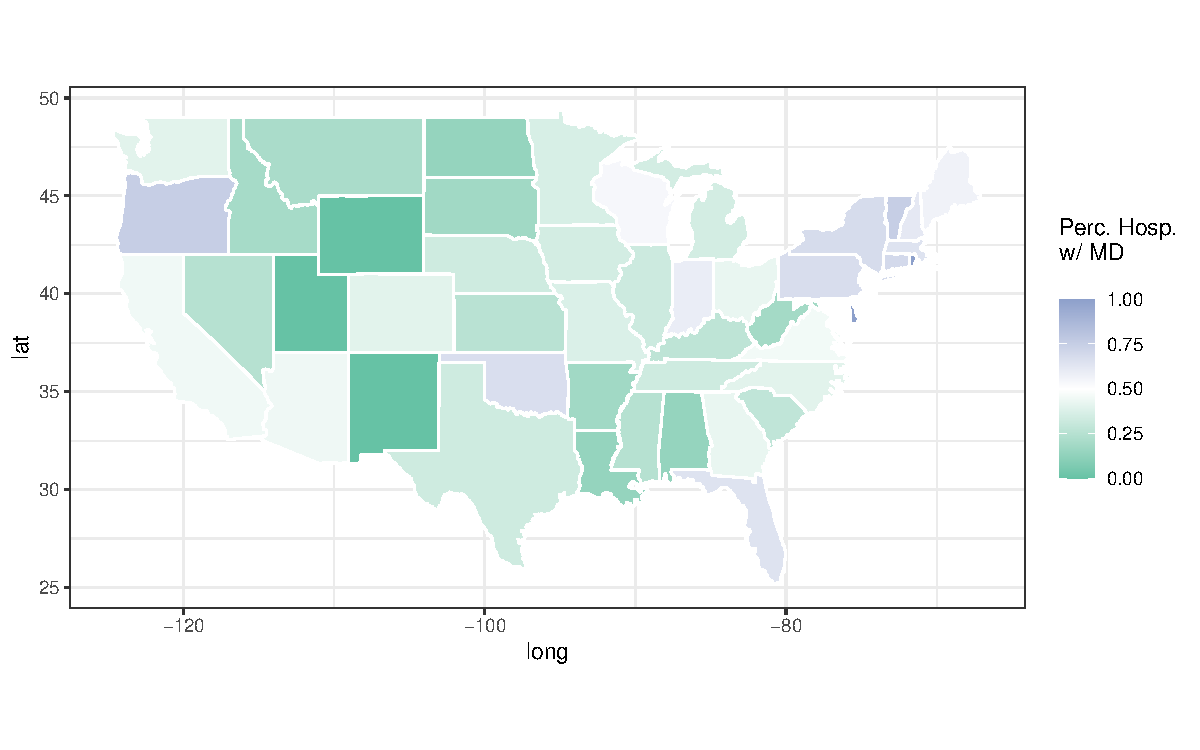
\includegraphics[width=\textwidth]{Objects/has_doc_avg_map.pdf}
    \label{fig:state_doc}
\end{figure}

\section{Modelling Hospital Response to Pay-for-Performance}\label{sec:model}

    I model hospital behavior under two simplified worlds: one where quality does not directly affect profit, and one where it does. Pay-for-performance incentives essentially incorporate performance directly into a hospital's profit function (\cite{dranove2011health}). I directly model performance as quality of care, which is inversely related to readmission and mortality rates. While the literature speculates about the true form of NFP objective functions, we can generally think of hospitals choosing some linear combination of profit and societal benefit, without knowing how much weight the hospital places on each. Intuitively, a hospital that places only weight on profit (for-profit type) will only care about quality when it enters into the profit function, and therefore will respond more drastically to pay-for-performance than a hospital who already cared about quality through societal benefit before the incentives. Therefore, hospital responses to pay-for-performance incentives reveal information about their underlying preference on profit vs. societal outcomes. 

    To formalize this intuition, I specify the hospital objective function as a weighted average of profit and societal (or patient) outcomes and derive characteristics of the optimal quality. For simplicity, I abstract away from quality having a direct effect of quantity and price. Without any financial incentives to increase quality, hospital quality is decided by:  
    
    $$\max_{\theta}\hspace{2mm}\alpha\left[R - c_{\theta}(\theta) \right] + (1-\alpha) u(\theta),$$

    \noindent where $R$ is net revenue, $c_{\theta}(.)$ is an increasing cost function specific to quality $\theta$, $u(.)$ is extra utility gained from quality, which is increasing and concave in $\theta$, and $\alpha\in[0,1]$ captures the weight placed on profit vs. societal benefit. There is an implicit stay-open condition throughout the model. Taking the first order condition yields 

    $$(1-\alpha)u'(\theta) = \alpha c_{\theta}'(\theta),$$

    \noindent where marginal benefit equals marginal cost of increasing quality. Solving for $u'(\theta)$ and differentiating with respect to $\alpha$:

    $$\frac{du'(\theta)}{d\alpha} = \frac{1}{(1-\alpha)^2}c_{\theta}'(\theta) > 0.$$

    \noindent Thus, by the Implicit Function Theorem, 

    $$\frac{d\theta}{d\alpha} = \frac{du'(\theta)/d\alpha}{du'(\theta)/d\theta} < 0.$$

    \noindent That is, the more weight on profit, the lower quality of care chosen by the hospital.

    In a world with pay-for-performance incentives, which can either look like benefits from high quality (such as HVBP) or penalties for low quality (as in HRRP), quality directly affects revenue. Thus, $R(\theta)$ is an increasing function of $\theta$, and I assume that the marginal financial benefit of increasing quality is greater than the marginal cost ($R'(\theta)\geq c_{\theta}'(\theta))$. Thus, the new first order condition yields:

    $$u'(\theta) = \frac{\alpha}{1-\alpha} \left[c_{\theta}'(\theta)-R(\theta)\right] \leq 0.$$

    \noindent Taking the derivative of this with respect to $\alpha$,

    $$\frac{du'(\theta)}{d\alpha} = \frac{1}{(1-\alpha)^2}c_{\theta}'(\theta).$$

    Therefore, again using the Implicit Function Theorem,

    $$\frac{d\theta}{d\alpha} = \frac{du'(\theta)/d\alpha}{du'(\theta)/d\theta}\geq0.$$

    That is, all else equal, in a world with financial incentives on quality, quality is increasing with more weight placed on profit. I combine the results found in each scenario into one response function that depends on $\alpha$, where $\theta_2$ is quality under pay-for-performance incentives and $\theta_1$ is quality with no financial incentive to quality. That is, 

    \begin{align*}
        \frac{d\Delta\theta}{d\alpha}&=\frac{d(\theta_2-\theta_1)}{d\alpha}\\
        &=\frac{d\theta_2}{d\alpha}-\frac{d\theta_1}{d\alpha}\\
        &\geq 0.
    \end{align*}


    Hence, this model predicts that change in quality depends on how much weight the hospital places on profit vs. societal benefit. Particularly, hospitals with more weight on profit respond more than hospitals with more weight placed on societal benefit. In reality, $\alpha$ is unknown, except in the case of for-profits, who have revealed that they have a high $\alpha$ by their ownership status. However, not-for-profit behavior on average does not bring much clarity about their objectives. An observable and economically relevant characteristic of a hospital that could affect $\alpha$ is composition of their executive leadership team. Thus, I compare the response of for-profits and not-for-profits with different leadership teams to bring clarity on how this might point to underlying $\alpha$.


\section{Matched vs. Unmatched Not-for-Profits}\label{app:matched}

The sample of all NFP hospitals that I use for analysis consists of 852 hospitals. In the AHA data, there are 2,258 additional NFP hospitals that either were not matched to tax forms, did not exist in the tax form data, or did not have executive names in the tax forms. While it would be ideal to analyze all NFPs, a sample size of 852 firms is relatively large in the hospital executive literature. 

In this section, I compare the in-sample NFPs to the out-of-sample NFPs along observable measures. I present means and standard deviations of these measures in Table \ref{tab:nfp_sample_compare}. The in-sample NFPs are slightly larger in terms of beds and patients seen. They are also slightly more likely to be penalized or receive payments under the pay-for-performance incentives. However, average readmission and mortality rates are very similar, as well as case mix index. The largest difference in the two samples is that I under-represent NFP hospitals in systems. This is due to the nature of the tax form 990s, where systems often file one tax form for the entire system, making it difficult to discern the true managers of a specific hospital. Because of this, I drop hospitals from the sample who only have leadership information from a system tax form. 

\import{Tables}{NFP_sample_comparison.tex}


\section{Executive Team Changes}\label{app:changes}

Here, I present descriptive statistics of executive team changes. In Figure \ref{fig:change_graph}, I show the average rate of MD executives to total executives, the percent of hospitals who fire an MD, and the percent of hospitals who hire an MD. The fraction of MD executives remains stable over time at approximately .22. Similarly, the percent of hospitals who hire an MD over time remains stable at approximately 21\%. There is a small increase in the percent of hospitals who fire an MD in 2011, but even with this increase firing is not common and stable, ranging from 12\% to 13\%. 

\begin{figure}[ht!]
    \centering
    \caption{Executive Team Changes Over Time}
    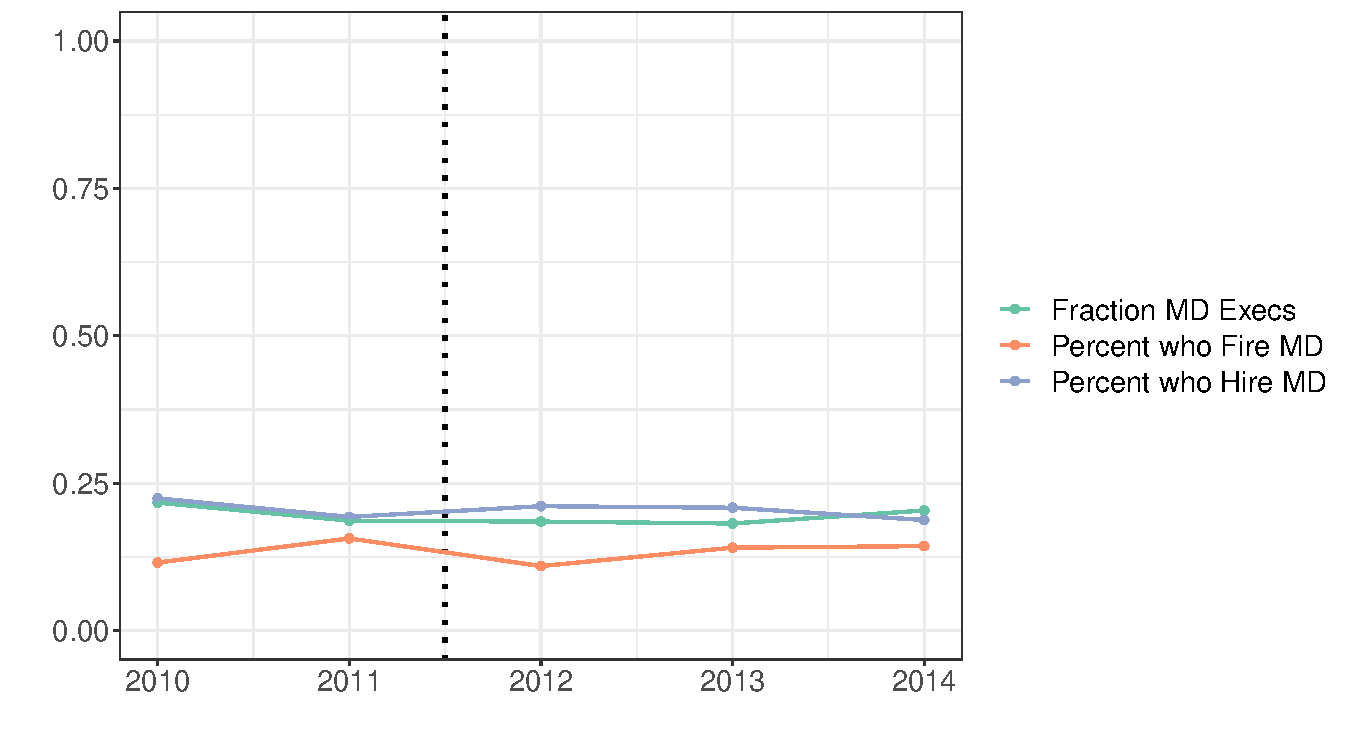
\includegraphics[width=\textwidth]{Objects/change_graph.pdf}
    \label{fig:change_graph}
\end{figure}

Additionally, I present the number of hospitals who change their propensity to hire a clinically trained executive at different times in Table \ref{tab:change_timing}. I break the timing up into pre-2012, 2012, and post-2012. I show the number of hospitals who have MDs in different time combinations. The number of hospitals that only have an MD executive in 2012, but at no other time, is only 6. The majority of hospitals (187) who ever have a clinical executive have one in every time period. 

\import{Tables}{change_num_table_2012.tex}

\section{Results By Condition}\label{app:condition}

The main results of the paper consider the weighted average readmission or mortality rate as the main outcomes. Here, I present results for each condition individually. Table \ref{tab:fp_read_condition_synth.tex}, I show the effect of being for-profit on AMI, heart failure, and pneumonia readmission rates compared to differing NFP comparison groups. The estimates indicate that the weighted average is mainly driven by pneumonia patients, since AMI readmission rate responses differ between FP and all NFP, where no other condition does. 

\import{Tables}{fp_read_condition_synth.tex}

Table \ref{tab:fp_mort_condition_synth.tex} shows a very similar result for mortality rates. AMI responses differ between FP and all NFP or NFP without clinical executives, but the weighted average is driven mainly by pneumonia patients. 

\import{Tables}{fp_mort_condition_synth.tex}

The differences between NFPs with and without clinical executives are also driven mainly by pneumonia patients, shown in Table \ref{tab:MD_noMD_readmort_condition_synth}.

\import{Tables}{MD_noMD_readmort_condition_synth.tex}

\section{TWFE Regression and Event Study Results}\label{app:fullsample}

While I ultimately employ a synthetic difference-in-differences framework, I also present the coefficient estimates and event study tables under a typical TWFE model specification. That is, there is no weighting of the control group or time periods. Table \ref{tab:forprofit_readmort_fullsample} shows coefficient estimates for the three specifications under Equation \ref{eq:forprofit}. Columns (1)-(3) show coefficient estimates for the weighted average readmission rate outcome, and columns (4)-(6) show coefficient estimates from the weighted average mortality outcome. Generally, these results are qualitatively identical to the synthetic difference-in-difference specification results. There is a statistically significant difference in readmission rate response between for-profits and NFPs with a clinical executive. Specifically, for-profits decrease their readmission rates by .4ppts more than NFPs with a clinical executive. There is no difference (statistically or in magnitude) between readmission rate responses of for-profits compared to all NFPs and NFPs without clincal executives. 

Similarly to the synthetic diff-in-diff estimates, there is no statistical difference in mortality between any of the hospital types, but the magnitude difference between for-profits and NFPs with clinical executives is much larger. This oculd be due to the noisiness of mortality as a measure. 

\import{Tables}{forprofit_readmort_fullsample.tex}

Further, I present coefficient estimates in Table \ref{tab:MD_noMD_readmort_fullsample} directly comparing NFPs with and without clinical executives for both readmission and mortality rates. Again, these results are very similar to the main results of the paper, with only slightly larger magnitudes. NFPs without a clinical executive respond to the pay-for-performance incentives by decreasing readmission and mortality rates more aggressively than NFPs with clinical executives. 

\import{Tables}{MD_noMD_readmort_fullsample.tex}

Finally, I present these results in typical event study form in Figure \ref{fig:es_plot}, which show no evidence of significant pre-trends driving the findings. 

\begin{figure}[ht!]
     \caption{TWFE Event Study Results}
     \centering
          \begin{subfigure}[b]{0.45\textwidth}
         \centering
         \caption{}
         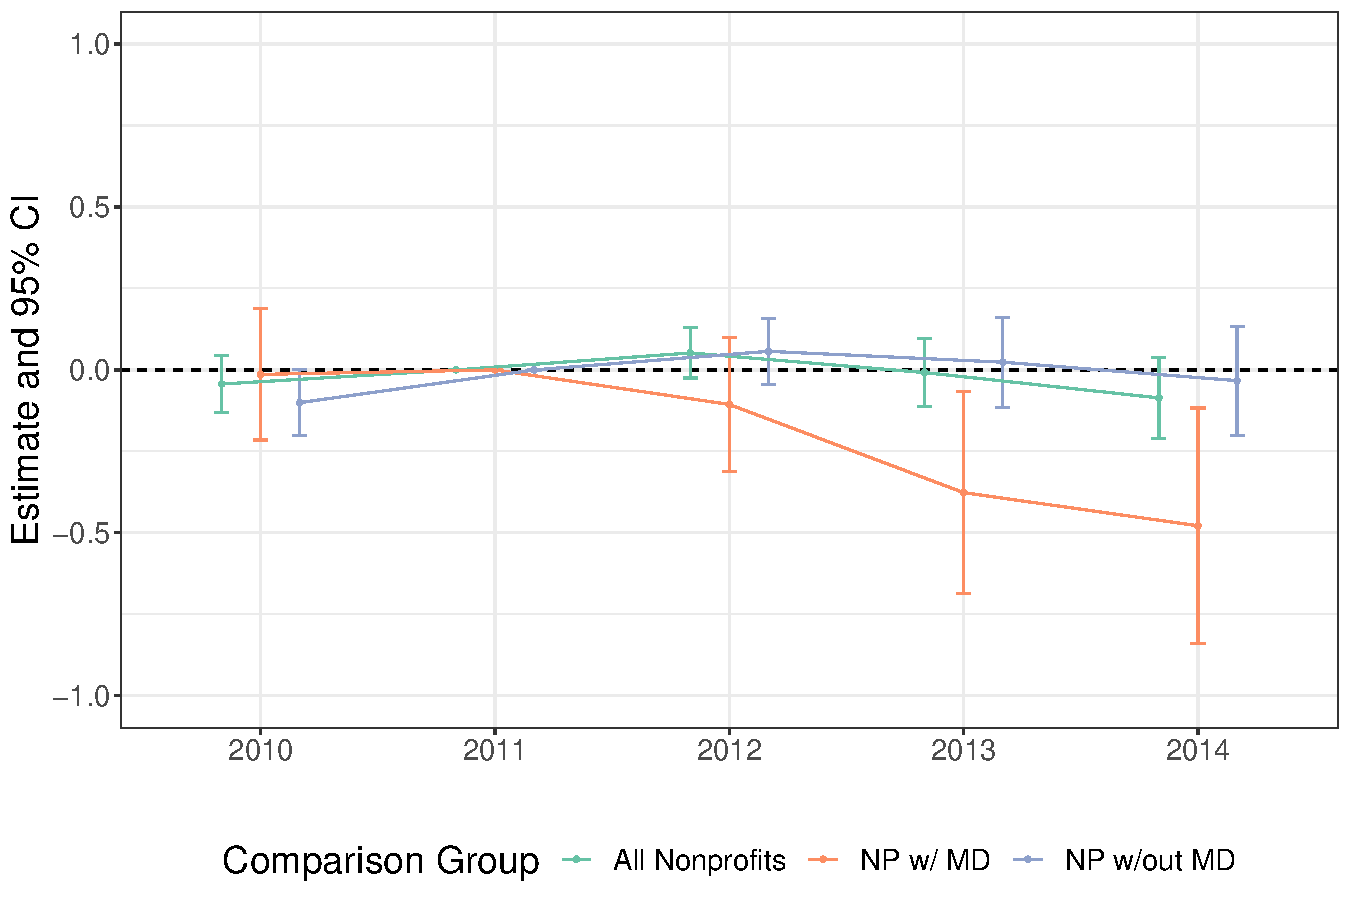
\includegraphics[width=\textwidth]{Objects/read_forprofit_es_graph.pdf}
         \label{fig:es_plota}
     \end{subfigure}%
     \hfill
     \begin{subfigure}[b]{0.45\textwidth}
         \centering
         \caption{}
         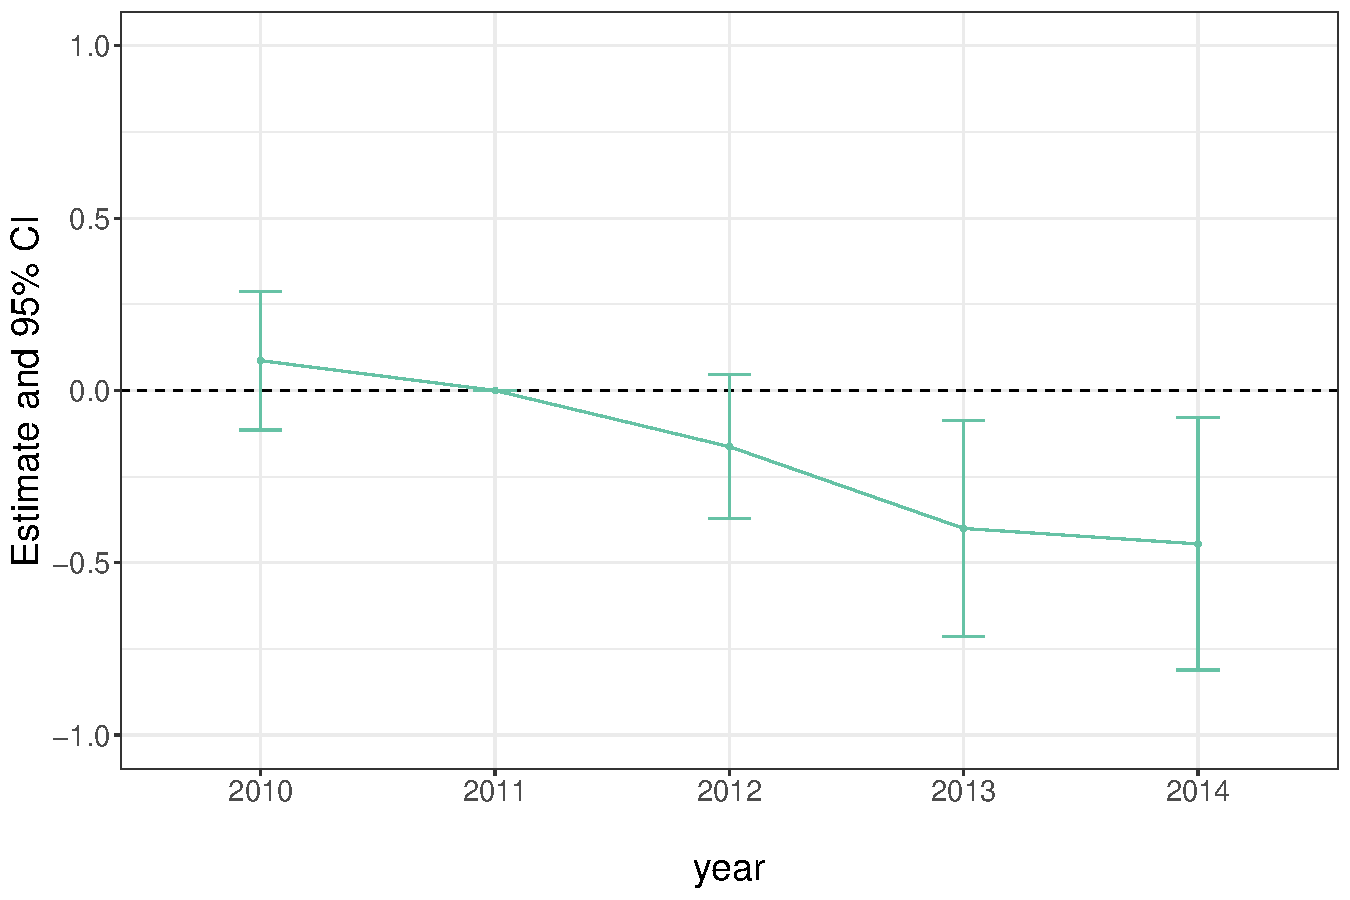
\includegraphics[width=\textwidth]{Objects/read_MD_es_graph.pdf}
         \label{fig:es_plotb}
     \end{subfigure}%
     \vspace{5mm}
     \hfill
     \begin{subfigure}[b]{0.45\textwidth}
         \centering
         \caption{}
         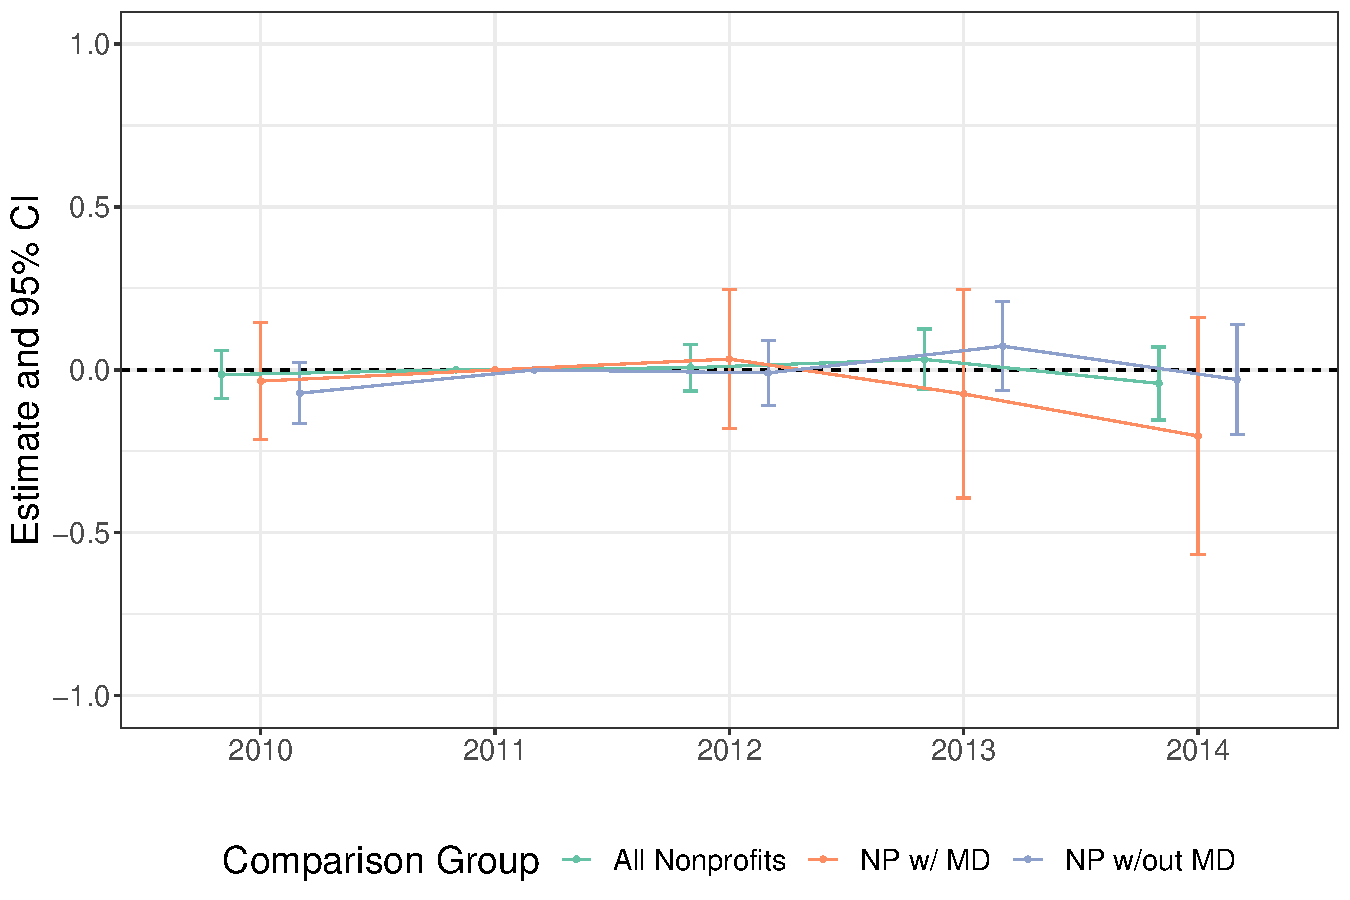
\includegraphics[width=\textwidth]{Objects/mort_forprofit_es_graph.pdf}
         \label{fig:es_plotc}
     \end{subfigure}
     \hfill
     \begin{subfigure}[b]{0.45\textwidth}
         \centering
         \caption{}
         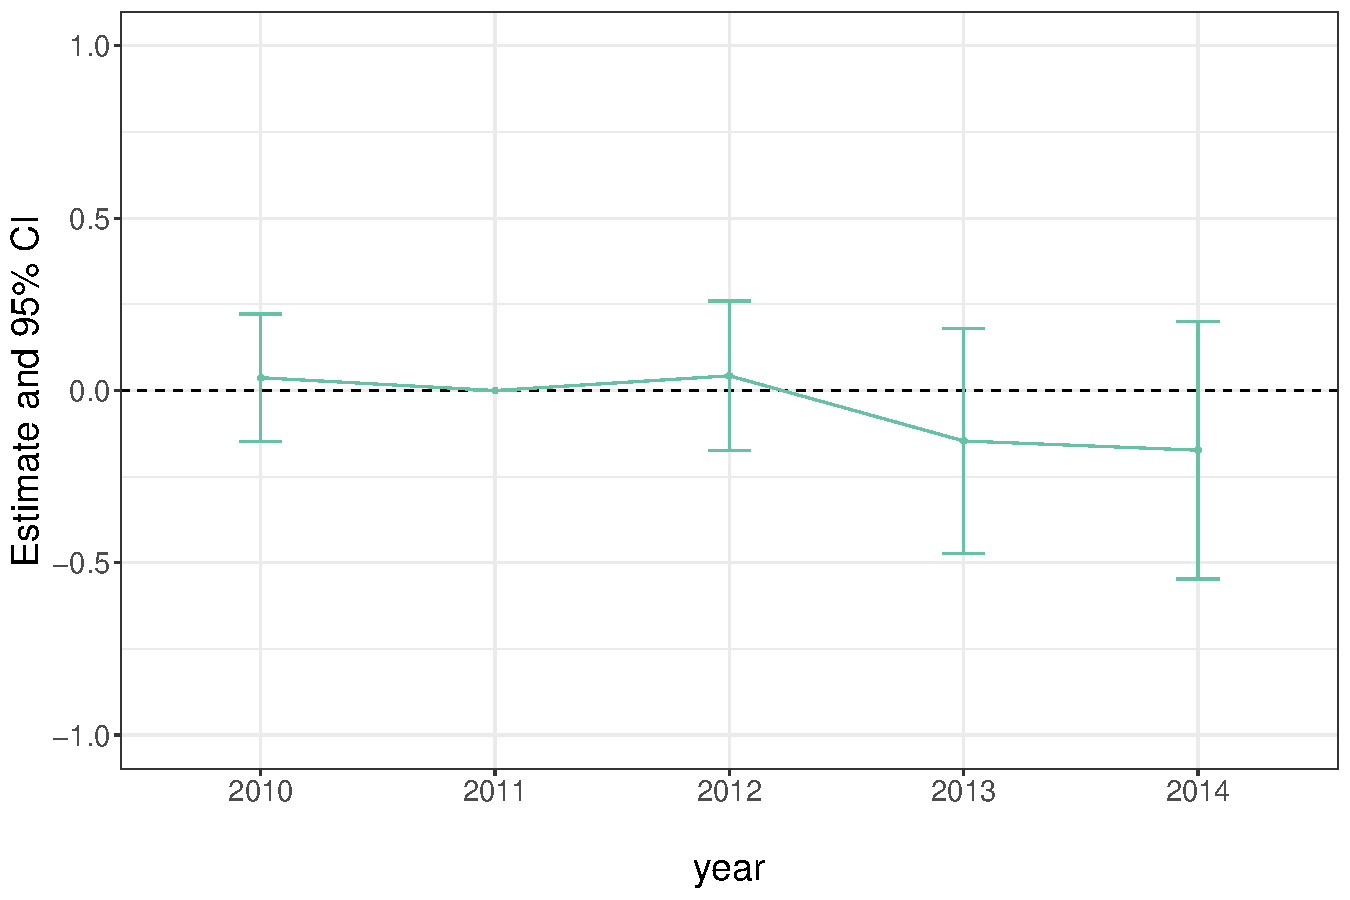
\includegraphics[width=\textwidth]{Objects/mort_MD_es_graph.pdf}
         \label{fig:es_plotd}
     \end{subfigure}
        \label{fig:es_plot}
    \end{figure}




\section{Synthetic Difference-in-Difference Coefficient Tables}

While I present the graphical representation of results in the main text, I also present a table of coefficients and standard errors for readmission and mortality rates in Tables \ref{tab:forprofit_readmort_synth} and \ref{tab:MD_noMD_readmort_synth}.

\import{Tables}{forprofit_readmort_synth.tex}

\import{Tables}{MD_noMD_readmort_synth.tex}


    

    

    

    

    

    

	
	
	


\end{document}

